\chapter{Atomic physics: Experimental techniques and theory}\label{chap:atomic_physics}

\begin{itemize}
\item Descriptions of the relevant physics in atomic physics experiments: Doppler cooling and magneto-optical traps, Sisyphus cooling, dipole forces, Feshbach resonances, scattering theory, Bose–Einstein statistics. Show how the Hamiltonian of a `two level' (32 levels, all things considered for $^{87}$Rb D line) atom with fine structure, hyperfine structure and Zeeman splitting arises from consideration of the different angular momenta. Use this to derive the differential equations for the state populations of an atom in a driving laser field. Gross Pitaevskii equation for single species, dual species and spinor condensate.

\item{Doppler cooling}
\item{Magneto-optical trapping}
\item{Optical dipole trapping}
\item{Two-body scattering and Feshbach resonances}
\item{ -> Include stuff from 3rd year report}
\item{Spin, fine structure, and hyperfine structure}
\item{Equations of motion for two level atom with hyperfine structure}
\item{The Monte-Carlo wavefunction method}
\item{Mean field theory for Bose–Einstein condensates}
\item{ -> Superfluid velocity}
\item{ -> Vortices}

\end{itemize}
\subsection{Experimental techniques}
\textsc{Bec}s provide such a tantalising opportunity for studying quantum phenomena not only because of their interesting properties, but also because of the level of control they afford. Many of the same techniques which allow experimentalists such control over their creation are also employed in the creation thereof, and many were discovered along the way to Bose--Einstein condensation.

The main experimental techniques used to create \bec---and which we are and will be employing in that pursuit---are Doppler cooling, magneto-optical and dipole trapping, polarisation gradient (Sisyphus) cooling, and evaporative cooling.

These were discovered, perhaps by no coincidence, in roughly the same order as they are called for in a \bec\ experiment.

\subsubsection{Doppler cooling}

Doppler cooling, demonstrated in 1978 \cite{wineland_radiation-pressure_1978} is a consequence of the simple observation that atoms see the wavelength of incident light Doppler shifted depending on their velocity. This can be used to selectively transfer momentum to only fast-moving atoms, by tuning an incident laser slightly redder than would be required for a resonant absorption. If six lasers in counterpropagating pairs orthogonal to each other surround a cloud of atoms, the atoms can be cooled close to the \emph{Doppler limit} \cite[p 58]{metcalf_laser_1999}

\begin{equation}
k_\up{B} T_\up{D} = \frac{\hbar\Gamma}2
\end{equation}

where $\Gamma$ is the linewidth of the atomic transition. For the cooling transition used for Doppler cooling $^{87}$Rb\footnote{The D$_2$ line, $5\up{S}_{\frac12}\rightarrow$ $5\up{P}_{\frac32}$, approximately 780 nm.}, this gives $146\,\upmu$K, which is approximately a factor of a thousand too high for Bose-condensation. These atoms are also not trapped.

\subsubsection{Magneto-optical and magnetic trapping}

Magneto-optical trapping, first demonstrated in 1987 \cite{raab_trapping_1987} comes from the realisation that a magnetic field can be used to \emph{spatially} vary the detuning from resonance that the atoms in the above mentioned arrangement of lasers see. This is possible due to the Zeeman effect \cite{zeeman_influence_1897}, in which the wavelengths of atomic transitions are shifted in a magnetic field.

If a field profile can be found which causes the transition to come closer to resonance as the atoms move away from a central point, then it forms a trap---atoms  that stray too far from the center will absorb more strongly and be deflected back\footnote{The polarisations of the beams are such that absorption from the inward facing beam occurs, rather than from the one that would accelerate the atom further outward!}.

The field configuration used in an anti-Helmholtz one, with two coils opposite each other carrying opposing currents. The resulting magnetic field profile has a zero in the middle and increases in magnitude in all directions.

With the Doppler beams off, this magnetic field still provides a trapping potential, due to the magnetic dipole interaction:

\begin{equation}
V(\vec{r}) = -\vec \mu \cdot \vec B,
\end{equation}
where $\vec\mu$ is the atomic magnetic moment, and $\vec B$ the magnetic field. This only traps some atomic spin states, and has losses due to spin-flips \cite{brink_majorana_2006} near the field zero.

\subsubsection{Optical trapping}

Optical dipole trapping on the other hand relies on the \emph{dipole force}, in which off-resonant light shifts the energy of the eigenstates of the combined atom-light system, the so called \emph{dressed states}. This energy shift, called the \emph{light shift}, depends on the intensity of the light, and so results in a potential that spatially varies as the intensity of the light. In the limit of large detuning (compared to Rabi frequency), this shift is given by \cite[p 8]{metcalf_laser_1999}:

\begin{equation}
\Delta E = \frac{\hbar\Omega^2}{4\delta}
\end{equation}

where $\delta$ is the detuning from resonance and the Rabi frequency is:
\begin{equation}
\Omega=\frac{eE_0}\hbar\langle1|\vec{x}|2\rangle,
\end{equation}

where $E_0$ is the amplitude of the light's electric field and  $\langle1|\vec{x}|2\rangle$ is the dipole moment between the two states in a two-level system.

With the potential proportional to $E_0^2$, and thus the light's intensity, the force the atom experiences is proportional to the light's intensity gradient. For this reason, the dipole force is also called the \emph{gradient force}. The name \emph{dipole force} comes from the fact that the force can be equivalently understood to arise from the polarisability of atoms in a light field, giving rise to a force identical to that which traps polarisable materials in optical tweezers \cite{ashkin_acceleration_1970}.

\subsubsection{Polarisation gradient cooling}

Polarisation gradient cooling, also called Sisyphus cooling, was proposed in 1989 \cite{dalibard_laser_1989, ungar_optical_1989} to explain experimentally measured cold atom cloud temperatures \cite{lett_optical_1989} which, at \textsc{nist} in 1988, were found to be well below the expected limit obtainable by the well understood method of Doppler cooling\footnote{As well as to explain other discrepancies between experiments and the theory of Doppler cooling, such as the optimal detuning of light being much greater than predicted.}, one of the few examples of experiments turning out better than expected. A one dimensional theory has been developed \cite{dalibard_laser_1989} which has found remarkable agreement with three dimensional experiments \cite{salomon_laser_1990}

One common configuration for Sisyphus cooling comprises two counterpropagating laser beams in each spatial dimension, both linearly polarised but with their polarisation angles perpendicular to one another. The optical field resulting from the two beams' superposition has regions of linear polarisation and of both helicities of circular polarisation, and varies between them on a length scale shorter than an optical wavelength.

The effect on multi-level atoms as they move from regions of one circular polarisation to another is that they are pumped alternately from one extreme of their spin-projection states to the other, alternately climbing and descending potential hills due to the dipole forces from the regions of different polarisations\footnote{If you consider only one polarisation of light, its intensity varies sinusoidally in space, creating a series of potential hills and wells via the dipole force}. And so, like the Greek legend of Sisyphus\footnote{Polarisation gradient cooling is but one of a family of so called `Sisyphus cooling' methods, all of which involve atoms repeatedly climbing potential hills.}, who was doomed to push a rock uphill for eternity, the atoms are climbing hills repeatedly. Due to the state dependence of the strength of the dipole forces, the atoms climb steeper hills than they descend, and are thus slowed and cooled.

This type of cooling does not work in a magnetic field; the splitting of transition frequencies makes it impossible for an atom to traverse its spin manifold on one laser frequency. For this reason the Sisyphus cooling stage is performed with magnetic fields off, though a sufficiently short period is required such that the atoms can be recaptured when the trapping field is restored.

\subsubsection{Evaporative cooling}

The final stage of cooling is forced \textsc{rf} evaporative cooling \cite{hess_evaporative_1986, anderson_observation_1995}, which decreases the temperature of the cloud by systematically removing the hottest atoms. This is performed in a magnetic trap, which as mentioned earlier, only traps certain spin states. Evaporation proceeds by using an \emph{\rf\ knife} to induce spin flips in the atoms. The \textsc{rf} frequency is chosen such that is is only resonant with atoms some distance away from the center of the trap (via the Zeeman shift). The furthest out atoms are the most energetic, possessing the energy to climb the magnetic potential the furthest. By flipping their spins, these atoms are ejected due to the magnetic field becoming anti-trapping for them.

The cloud is given some time to rethermalise and the knife\footnote{So called because it cuts the tail off the velocity distribution of the atom cloud.} is moved inward where it removes slightly colder atoms. This is repeated until the desired compromise of lower temperature/lower atom number is reached. Usually some method is employed to prevent atoms near the center of the trap from undergoing spin flips \cite{brink_majorana_2006} as they move across the field zero. The method we'll employ is to use an optical dipole trap in combination with the magnetic trap \cite{lin_rapid_2009}, such that the coldest atoms get trapped in the dipole trap which is offset from the magnetic field zero.

\subsubsection{The Gross-Pitaevskii equation and Vortices}

Bose-condensates are described well by \emph{mean field} theory, whereby the many-body wavefunction is approximated by a product of identical single-particle wavefunctions. Indeed, that the majority of the atoms are in the same quantum state is one of the defining features of \bec. The effect of interparticle interactions is included as a nonlinear term in the Schr\"odinger equation for the single particle wavefunctions, known as the Gross-Pitaevskii equation:

\begin{equation}
\frac{\partial \Psi}{\partial t} = \left[-\frac{\hbar^2}{2m}\nabla^2 + V(\vec{x}) + g|\Psi|^2\right]\Psi,
\end{equation}

where $g$ characterises the strength of the interparticle interactions\footnote{And is usually positive---having the effect of stabilising \bec s by self-repulsion.}, and $\Psi = \sqrt{N}\Psi_\up{single}$ is the single-particle wavefunction scaled by the square root of the number of particles\footnote{Thus giving it the property that $|\Psi|^2$ is the particle density.}.

In the hydrodynamic formulation of quantum mechanics \cite{madelung_quantentheorie_1927}, the flow velocity of a spatial wavefunction can be defined by considering the probability current to be a product of density and velocity. This allows us to define the superfluid velocity of a \bec\ as:
\begin{equation}
\vec v = \frac\hbar m \nabla\phi
\end{equation}
where $\phi$ is the phase of the condensate wavefunction $\Psi$. Integrating this velocity over any closed path $\gamma$ gives us the circulation:

\begin{align}
C &= \frac\hbar m\oint_\gamma\nabla\phi\,ds\\
  &= \frac\hbar m 2\pi n.\qquad n=0,1,2\dots
\end{align}
The fact that the circulation is quantised means that vorticity cannot exist in the condensate except in one-dimensional lines, about which the wavefunction's phase winds by a multiple of $2\pi$. These topological defects are the quantised vortices that are central to this project.

At a vortex core, the atom density of a \bec\ must go to zero. This can be intuitively understood to arise from centrifugal forces, but is also required in order for the wavefunction to be continuous and single-valued across the core. This drop in density in the vicinity of a vortex core is what our method exploits in order to trap atoms within the cores.

\subsubsection{Feshbach resonances}

A Feshbach resonance \cite{chin_feshbach_2010} is an enhancement of the interparticle interaction strength when when a certain magnetic field strength is applied\footnote{Feshbach resonances can also be induced optically and with \rf\, but magnetic resonances are the most commonly used.}. This phenomenon was first discovered in ultracold atoms in 1998 \cite{inouye_observation_1998}, and is now a staple of cold atom experiments.

\begin{figure}%[htb]
\begin{center}
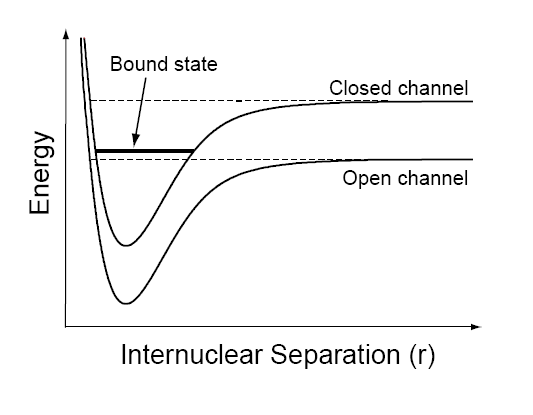
\includegraphics[width=0.5\textwidth]{figures/unsorted/feshbach.png}
\caption{When atoms approach each other with spins aligned, they are in the \emph{open channel}. In this channel they are unbound, but do not have enough energy to be free in the other channel - the \emph{closed channel}. In the close range however, the atoms may have energy corresponding to a bound (molecular) state of the closed channel, a resonance which causes a divergence in the scattering length. The energy difference between the two channels can be tuned with a magnetic field and so these resonances can be induced in a wide range of situations.}\label{fig:feshbach}
\end{center}
\end{figure}
The interparticle interaction mentioned above:

\begin{equation}
g = \frac{2\pi \hbar^2 a}{m_r}
\end{equation}
where $m_r$ is the reduced mass of a pair of the interacting particles, is dependent on a parameter $a$ called the \emph{s-wave scattering length}, which characterises low energy collisions between atoms. It is sensitive not only to what species of atoms are colliding, but also to their spin states. For each combination of spins, there is a different inter-atomic potential (called a \emph{channel}) which determines the collision dynamics (Figure \ref{fig:feshbach}).

The resulting scattering length is sensitive to any bound states of this inter-atomic potential which are near the collision energy. If the channels of different spin states are coupled via the hyperfine interaction\footnote{Requiring that the atoms in question have a nuclear magnetic moment.}, then the scattering length is also sensitive to bound states in the channels other the one the atoms are in when they are far from each other. Due to the Zeeman effect, the energies between the different channels can be shifted with a magnetic field, and so a bound state can be shifted close to the collision energy, which causes the scattering length to diverge.

The end result is that at certain magnetic field strengths we find that atoms are much more strongly attracted to or repelled from each other.

\begin{figure}%[htb]
\begin{center}
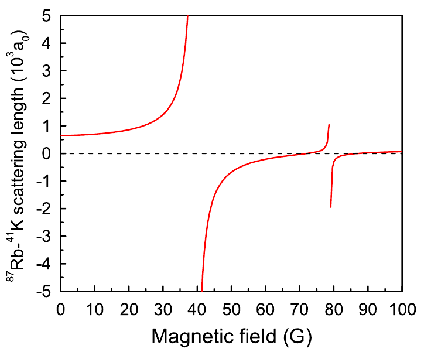
\includegraphics[width=0.5\textwidth]{figures/unsorted/feshKRb.png}
\caption{Predicted interspecies scattering length \cite{thalhammer_double_2008} as a function of magnetic field strength, for $^{41}$K and $^{87}$Rb both in their lowest energy hyperfine groundstate. The 35 gauss resonance is one of the main reasons for this pair of atoms being used in this project. It has a particularly low field strength and large width compared to most Feshbach resonances.}\label{fig:feshKRb}
\end{center}
\end{figure}

We plan to use a Feshbach resonance (Figure \ref{fig:feshKRb}) to enhance the interspecies repulsion between $^{87}$Rb and $^{41}$K, thus trapping tracer particles more strongly in vortex cores.
